

\tikzset{every picture/.style={line width=0.75pt}} %set default line width to 0.75pt        

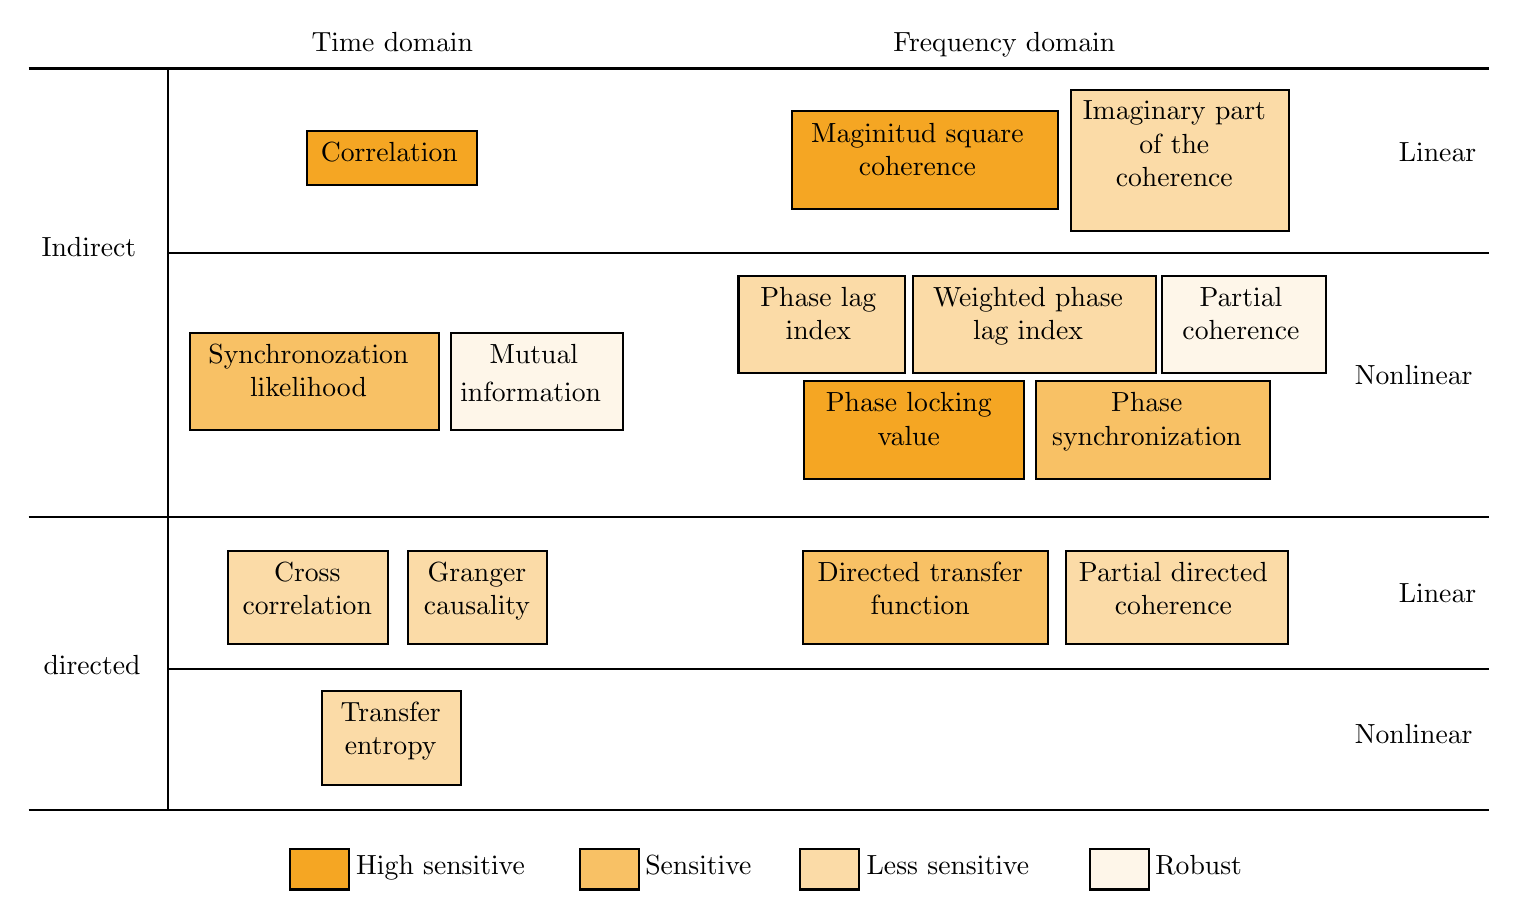
\begin{tikzpicture}[x=0.75pt,y=0.75pt,yscale=-1,xscale=1]
%uncomment if require: \path (0,433); %set diagram left start at 0, and has height of 433





%Shape: Rectangle [id:dp19082824282694832] 
\draw  [fill={rgb, 255:red, 245; green, 166; blue, 35 }  ,fill opacity=1 ] (123.2,395.72) -- (151.65,395.72) -- (151.65,415.39) -- (123.2,415.39) -- cycle ;
%Shape: Rectangle [id:dp05778591761365015] 
\draw  [fill={rgb, 255:red, 245; green, 166; blue, 35 }  ,fill opacity=0.7 ] (262.86,395.72) -- (291.3,395.72) -- (291.3,415.39) -- (262.86,415.39) -- cycle ;
%Shape: Rectangle [id:dp582586865477011] 
\draw  [fill={rgb, 255:red, 245; green, 166; blue, 35 }  ,fill opacity=0.4 ] (368.86,395.72) -- (397.3,395.72) -- (397.3,415.39) -- (368.86,415.39) -- cycle ;
%Shape: Rectangle [id:dp2934828137943699] 
\draw  [fill={rgb, 255:red, 245; green, 166; blue, 35 }  ,fill opacity=0.1 ] (508.86,395.72) -- (537.3,395.72) -- (537.3,415.39) -- (508.86,415.39) -- cycle ;

%Straight Lines [id:da8160435757030788] 
\draw    (64.43,108.67) -- (701.13,108.67) ;
%Straight Lines [id:da9069272127277761] 
\draw    (-2.64,236) -- (701.13,236) ;
%Straight Lines [id:da10616872455225357] 
\draw    (64.43,309.22) -- (701.13,309.22) ;
%Straight Lines [id:da8429859579606707] 
\draw    (-2.64,377.22) -- (701.13,377.22) ;
%Straight Lines [id:da004185251792945044] 
\draw    (-2.64,19.83) -- (701.13,19.83) ;
%Straight Lines [id:da6602898765459473] 
\draw    (64.43,20.67) -- (64.43,377.22) ;

% Text Node
\draw (27.86,301.22) node [anchor=north] [inner sep=0.75pt]   [align=left] {directed};
% Text Node
\draw (26.36,99.67) node [anchor=north] [inner sep=0.75pt]   [align=left] {Indirect};
% Text Node
\draw (172.5,0.67) node [anchor=north] [inner sep=0.75pt]   [align=left] {Time domain};
% Text Node
\draw (467.37,0.67) node [anchor=north] [inner sep=0.75pt]   [align=left] {Frequency domain};
% Text Node
\draw  [color={rgb, 255:red, 0; green, 0; blue, 0 }  ,draw opacity=1 ][fill={rgb, 255:red, 245; green, 166; blue, 35 }  ,fill opacity=1 ]  (131.5,50) -- (213.5,50) -- (213.5,76) -- (131.5,76) -- cycle  ;
\draw (134.5,54) node [anchor=north west][inner sep=0.75pt]  [color={rgb, 255:red, 0; green, 0; blue, 0 }  ,opacity=1 ] [align=left] {\begin{minipage}[lt]{52.62pt}\setlength\topsep{0pt}
\begin{center}
Correlation
\end{center}

\end{minipage}};
% Text Node
\draw (676.13,54) node [anchor=north] [inner sep=0.75pt]   [align=left] {Linear};
% Text Node
\draw  [color={rgb, 255:red, 0; green, 0; blue, 0 }  ,draw opacity=1 ][fill={rgb, 255:red, 245; green, 166; blue, 35 }  ,fill opacity=1 ]  (365.17,40.5) -- (493.17,40.5) -- (493.17,87.5) -- (365.17,87.5) -- cycle  ;
\draw (368.17,44.5) node [anchor=north west][inner sep=0.75pt]  [color={rgb, 255:red, 0; green, 0; blue, 0 }  ,opacity=1 ] [align=left] {\begin{minipage}[lt]{83.8pt}\setlength\topsep{0pt}
\begin{center}
Maginitud square \\coherence
\end{center}

\end{minipage}};
% Text Node
\draw  [color={rgb, 255:red, 0; green, 0; blue, 0 }  ,draw opacity=1 ][fill={rgb, 255:red, 245; green, 166; blue, 35 }  ,fill opacity=0.4 ]  (499.53,30) -- (604.53,30) -- (604.53,98) -- (499.53,98) -- cycle  ;
\draw (502.53,34) node [anchor=north west][inner sep=0.75pt]  [color={rgb, 255:red, 0; green, 0; blue, 0 }  ,opacity=1 ] [align=left] {\begin{minipage}[lt]{67.92pt}\setlength\topsep{0pt}
\begin{center}
Imaginary part\\of the\\coherence
\end{center}

\end{minipage}};
% Text Node
\draw  [color={rgb, 255:red, 0; green, 0; blue, 0 }  ,draw opacity=1 ][fill={rgb, 255:red, 245; green, 166; blue, 35 }  ,fill opacity=1 ]  (370.83,170.56) -- (476.83,170.56) -- (476.83,217.56) -- (370.83,217.56) -- cycle  ;
\draw (373.83,174.56) node [anchor=north west][inner sep=0.75pt]  [color={rgb, 255:red, 0; green, 0; blue, 0 }  ,opacity=1 ] [align=left] {\begin{minipage}[lt]{69.06pt}\setlength\topsep{0pt}
\begin{center}
Phase locking \\value
\end{center}

\end{minipage}};
% Text Node
\draw  [color={rgb, 255:red, 0; green, 0; blue, 0 }  ,draw opacity=1 ][fill={rgb, 255:red, 245; green, 166; blue, 35 }  ,fill opacity=0.4 ]  (339.33,119.69) -- (419.33,119.69) -- (419.33,166.69) -- (339.33,166.69) -- cycle  ;
\draw (342.33,123.69) node [anchor=north west][inner sep=0.75pt]  [color={rgb, 255:red, 0; green, 0; blue, 0 }  ,opacity=1 ] [align=left] {\begin{minipage}[lt]{50.92pt}\setlength\topsep{0pt}
\begin{center}
Phase lag \\index
\end{center}

\end{minipage}};
% Text Node
\draw  [color={rgb, 255:red, 0; green, 0; blue, 0 }  ,draw opacity=1 ][fill={rgb, 255:red, 245; green, 166; blue, 35 }  ,fill opacity=0.4 ]  (423.5,119.69) -- (540.5,119.69) -- (540.5,166.69) -- (423.5,166.69) -- cycle  ;
\draw (426.5,123.69) node [anchor=north west][inner sep=0.75pt]  [color={rgb, 255:red, 0; green, 0; blue, 0 }  ,opacity=1 ] [align=left] {\begin{minipage}[lt]{76.25pt}\setlength\topsep{0pt}
\begin{center}
Weighted phase\\lag index
\end{center}

\end{minipage}};
% Text Node
\draw  [color={rgb, 255:red, 0; green, 0; blue, 0 }  ,draw opacity=1 ][fill={rgb, 255:red, 245; green, 166; blue, 35 }  ,fill opacity=0.1 ]  (543.33,119.69) -- (622.33,119.69) -- (622.33,166.69) -- (543.33,166.69) -- cycle  ;
\draw (546.33,123.69) node [anchor=north west][inner sep=0.75pt]  [color={rgb, 255:red, 0; green, 0; blue, 0 }  ,opacity=1 ] [align=left] {\begin{minipage}[lt]{50.36pt}\setlength\topsep{0pt}
\begin{center}
Partial\\coherence
\end{center}

\end{minipage}};
% Text Node
\draw  [color={rgb, 255:red, 0; green, 0; blue, 0 }  ,draw opacity=1 ][fill={rgb, 255:red, 245; green, 166; blue, 35 }  ,fill opacity=0.1 ]  (200.79,147.06) -- (283.79,147.06) -- (283.79,194.06) -- (200.79,194.06) -- cycle  ;
\draw (203.79,151.06) node [anchor=north west][inner sep=0.75pt]  [color={rgb, 255:red, 0; green, 0; blue, 0 }  ,opacity=1 ] [align=left] {\begin{minipage}[lt]{53.18pt}\setlength\topsep{0pt}
\begin{center}
Mutual
\end{center}
information
\end{minipage}};
% Text Node
\draw  [color={rgb, 255:red, 0; green, 0; blue, 0 }  ,draw opacity=1 ][fill={rgb, 255:red, 245; green, 166; blue, 35 }  ,fill opacity=0.7 ]  (75.17,147.06) -- (195.17,147.06) -- (195.17,194.06) -- (75.17,194.06) -- cycle  ;
\draw (78.17,151.06) node [anchor=north west][inner sep=0.75pt]  [color={rgb, 255:red, 0; green, 0; blue, 0 }  ,opacity=1 ] [align=left] {\begin{minipage}[lt]{78.7pt}\setlength\topsep{0pt}
\begin{center}
Synchronozation\\likelihood
\end{center}

\end{minipage}};
% Text Node
\draw  [color={rgb, 255:red, 0; green, 0; blue, 0 }  ,draw opacity=1 ][fill={rgb, 255:red, 245; green, 166; blue, 35 }  ,fill opacity=0.7 ]  (482.5,170.56) -- (595.5,170.56) -- (595.5,217.56) -- (482.5,217.56) -- cycle  ;
\draw (485.5,174.56) node [anchor=north west][inner sep=0.75pt]  [color={rgb, 255:red, 0; green, 0; blue, 0 }  ,opacity=1 ] [align=left] {\begin{minipage}[lt]{73.6pt}\setlength\topsep{0pt}
\begin{center}
Phase\\synchronization
\end{center}

\end{minipage}};
% Text Node
\draw (664.63,161.56) node [anchor=north] [inner sep=0.75pt]   [align=left] {Nonlinear};
% Text Node
\draw  [color={rgb, 255:red, 0; green, 0; blue, 0 }  ,draw opacity=1 ][fill={rgb, 255:red, 245; green, 166; blue, 35 }  ,fill opacity=0.4 ]  (93.5,252.22) -- (170.5,252.22) -- (170.5,297.22) -- (93.5,297.22) -- cycle  ;
\draw (96.5,256.22) node [anchor=north west][inner sep=0.75pt]  [color={rgb, 255:red, 0; green, 0; blue, 0 }  ,opacity=1 ] [align=left] {\begin{minipage}[lt]{50.35pt}\setlength\topsep{0pt}
\begin{center}
Cross \\correlation
\end{center}

\end{minipage}};
% Text Node
\draw  [color={rgb, 255:red, 0; green, 0; blue, 0 }  ,draw opacity=1 ][fill={rgb, 255:red, 245; green, 166; blue, 35 }  ,fill opacity=0.4 ]  (180.17,252.22) -- (247.17,252.22) -- (247.17,297.22) -- (180.17,297.22) -- cycle  ;
\draw (183.17,256.22) node [anchor=north west][inner sep=0.75pt]  [color={rgb, 255:red, 0; green, 0; blue, 0 }  ,opacity=1 ] [align=left] {\begin{minipage}[lt]{42.97pt}\setlength\topsep{0pt}
\begin{center}
Granger \\causality
\end{center}

\end{minipage}};
% Text Node
\draw (676.13,266.72) node [anchor=north] [inner sep=0.75pt]   [align=left] {Linear};
% Text Node
\draw  [color={rgb, 255:red, 0; green, 0; blue, 0 }  ,draw opacity=1 ][fill={rgb, 255:red, 245; green, 166; blue, 35 }  ,fill opacity=0.7 ]  (370.33,252.22) -- (488.33,252.22) -- (488.33,297.22) -- (370.33,297.22) -- cycle  ;
\draw (373.33,256.22) node [anchor=north west][inner sep=0.75pt]  [color={rgb, 255:red, 0; green, 0; blue, 0 }  ,opacity=1 ] [align=left] {\begin{minipage}[lt]{78.12pt}\setlength\topsep{0pt}
\begin{center}
Directed transfer\\function
\end{center}

\end{minipage}};
% Text Node
\draw  [color={rgb, 255:red, 0; green, 0; blue, 0 }  ,draw opacity=1 ][fill={rgb, 255:red, 245; green, 166; blue, 35 }  ,fill opacity=0.4 ]  (497.2,252.22) -- (604.2,252.22) -- (604.2,297.22) -- (497.2,297.22) -- cycle  ;
\draw (500.2,256.22) node [anchor=north west][inner sep=0.75pt]  [color={rgb, 255:red, 0; green, 0; blue, 0 }  ,opacity=1 ] [align=left] {\begin{minipage}[lt]{70.76pt}\setlength\topsep{0pt}
\begin{center}
Partial directed\\coherence
\end{center}

\end{minipage}};
% Text Node
\draw  [color={rgb, 255:red, 0; green, 0; blue, 0 }  ,draw opacity=1 ][fill={rgb, 255:red, 245; green, 166; blue, 35 }  ,fill opacity=0.4 ]  (138.5,319.83) -- (205.5,319.83) -- (205.5,364.83) -- (138.5,364.83) -- cycle  ;
\draw (141.5,323.83) node [anchor=north west][inner sep=0.75pt]  [color={rgb, 255:red, 0; green, 0; blue, 0 }  ,opacity=1 ] [align=left] {\begin{minipage}[lt]{43.15pt}\setlength\topsep{0pt}
\begin{center}
Transfer \\entropy
\end{center}

\end{minipage}};
% Text Node
\draw (664.63,334.33) node [anchor=north] [inner sep=0.75pt]   [align=left] {Nonlinear};
% Text Node
\draw (153.66,397.56) node [anchor=north west][inner sep=0.75pt]   [align=left] {High sensitive};
% Text Node
\draw (292.93,397.56) node [anchor=north west][inner sep=0.75pt]   [align=left] {Sensitive};
% Text Node
\draw (399.59,397.56) node [anchor=north west][inner sep=0.75pt]   [align=left] {Less sensitive};
% Text Node
\draw (538.66,397.56) node [anchor=north west][inner sep=0.75pt]   [align=left] {Robust};


\end{tikzpicture}
